\chapter{Background}
\label{background}

\section{Introduction}
\label{background_intro}
RAPID's connected DSSs make use of spatial data;\footnote{\textit{Spatial} versus \textit{geospatial} terminology: Some groups make a subtle distinction between spatial data and geospatial data. In those cases, spatial data describes data ``distributed in three-dimensional space,'' with ``measurable'' dimensions~\cite{Bhatta2011}. Given \textit{geography}'s definition, geospatial data is ``spatial data which is related to the Earth''~\cite{Bhatta2011}. In this thesis, spatial data is always located on Earth, so \textit{spatial} and \textit{geospatial} will be used interchangeably. As one supporting source, the United States Geological Survey considers ``the terms spatial and geospatial [to be] equivalent.''
\cite{Bhatta2011}} their eventual goal is to lay out and recommend pipeline routes through areas with as few hazards as possible~\cite{Dunning2013}. As such, this end-to-end system can be considered a spatial DSS (SDSS). SDSSs are uniquely tasked with providing ``easy access to spatial data and decision models through the integration of spatial databases, analytical models, and visualization tools''~\cite{RedlandsSDSS}.

RAPID manages the spatial database component and also has to account for geographic information systems' (GIS) mathematical foundations. This chapter describes basic GIS concepts and requisite information for geospatial database management systems, structured and unstructured geospatial data, and related standards. These have all played into RAPID's motivations and implementation.

\subsection{Open Geospatial Consortium}
The Open Geospatial Consortium (OGC) is an international consortium---originating in 1994---with several hundred industry, government, and academic participants. Its goal is to establish standard formats and interfaces for geospatial data and applications. They've created over thirty-five standards, usually in the form of markup, modeling, or query languages as well as API specifications~\cite{ogc}.

Many organizations insist on using OGC-compliant products and services to promote robustness and interoperability. RAPID implements components of several OGC Standards. While not a top-to-bottom OGC-standardized system, RAPID is partway there and still useful because it builds on the same foundational concepts.

\section{GISs}
A GIS is a computer system (including hardware and software) for working with geographic data---that is, data associated with a location in space~\cite{Esriintro}. Quite simply, GISs provide a means of managing and analyzing this data. More importantly, GISs allow people to understand deep, complex information about geographic locations, their relative positions, and the objects and conditions that are located there~\cite{Esriintro}.

Because many everyday and large-scale tasks and concerns are related to specific locations, so too are the computer applications that people use: flight scheduling and routing, car navigation, weather prediction, demographic analysis, social networking, economics, and politics~\cite{Esriintro}. RAPID and its related applications, with their geospatial data, enable similar uses.

\subsection{Functionality}
GIS functionality can usually be placed in one of five categories~\cite{Esriintro}:

\begin{description}
  \item[Mapping objects' locations] Descriptors can be assigned to points in space: for example, addresses. In a technical sense, this can usually be seen as associating string-like data---ideas or concepts (like place names)---with floating-point latitude and longitude. These are commonly called \textit{features} (central to any geospatial system).
  \item[Mapping quantities] Quantities can be mapped to certain points to relate locations to numeric data about them. This could be integers and floating point values, again, assigned to latitude and longitude. These can also be considered features.
  \item[Mapping densities] Not only can values be assigned to specific points on a map, densities can be generated and displayed, which show the distribution of objects or values over an area.
  \item[Determining objects' relative positions] GISs can determine if objects or locations are located inside or outside of other locations. Additionally, they measure distances between objects and locations and determine how near or far objects are.\footnote{This is the key to geospatial database management system design---looking up data based on spatial calculations quickly.}
  \item[Analyzing trends] Lastly, many GISs look at trends in data. There's a lot of demand and opportunity for analysis of how locations and features change over time.
\end{description}

In summary, GISs capture, manage, analyze, and display geographically-referenced information. Viewing and understanding relevant relationships, patterns, and trends can be done in the form of maps, globes, reports, and charts~\cite{Esriintro}. RAPID, at a low level, acts as a foundation for that functionality.

\section{Data characteristics}
The section outlines more technical design considerations for geospatial data, which isn't always easily represented or stored in common data formats. Although humans often represent points in space with numbers (and, occasionally, symbols) it's best to treat them as their own primitive data type in software~\cite{gentle_intro}.

Because of this, geospatial data structures and file formats must be able to specify points in two or three dimensions (usually latitude and longitude, and maybe elevation).\footnote{Conceptually, time can be viewed as an additional dimension---one of a feature's properties---so the data is geospatial-\textit{temporal}.} GISs and spatial database management systems often need to account for any arbitrary coordinate system~\cite{gentle_intro}.

Considering the above, two common file and data types have come about in GISs: vector and raster. They are briefly described below.

\subsubsection{Vector}
\label{sec:vector}
Vector files contain mathematical and geometric representations of spatial data---defining points and shapes in space. They are split into two components: (1) series of coordinate pairs and (2) attributes~\cite{gentle_intro}.

\paragraph{Coordinate pair series}
Coordinate pairs are two values that represent a point in space in a coordinate system. Most commonly, this is the geographic coordinate system, where one value is latitude and other value is latitude. Taken together, any point on Earth's surface can be represented~\cite{gentle_intro}.\footnote{Geographic projections and digital coordinate system specifications are a large area of study. RAPID cannot entirely ignore these considerations and distinctions, but once a few database and parser options are set, we can mostly set those concerns aside. This is discussed in Section~\ref{design_srid}.}

In vector files, sequences (or ``series'') of these points can represent different cartographic concepts. There are points, lines, linestrings, and polygons:

\begin{description}
  \item[Points] Points are single instances of the points described above: they represent a single point in space.
  \item[Lines] Lines are drawn from one point to another (and are represented by that pair of points).
  \item[Linestrings] Linestrings are multiple connected lines (and, thus, chained pairs of points). These can represent concepts like borders between countries or road networks.
  \item[Polygons] Polygons are linestrings where the last point is equal to the first point---creating a closed shape. Political borders in the United States are a good example: the country is broken up into states, and states are broken up into counties, cities, and congressional districts.
\end{description}

The above can be extended to include polygons with holes. Imagine mapping California's land: where there are bodies of water on the map, there are simply holes in the polygon~\cite{gentle_intro}.

\begin{figure}
    \centering

      \subfloat[Point]{\label{fig:a}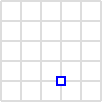
\includegraphics[width=0.2\textwidth]{figures/point.png}}
      \hfill
        \subfloat[Multipoint]{\label{fig:a}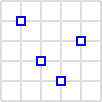
\includegraphics[width=0.2\textwidth]{figures/multipoint.png}}
        \hfill
\subfloat[Linestring]{\label{fig:a}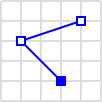
\includegraphics[width=0.2\textwidth]{figures/linestring.png}}
       \hfill
\subfloat[Multilinestring]{\label{fig:a}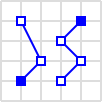
\includegraphics[width=0.2\textwidth]{figures/multilinestring.png}}

      \subfloat[Polygon]{\label{fig:a}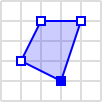
\includegraphics[width=0.2\textwidth]{figures/polygon.png}}
      \hfill
        \subfloat[Polygon with hole]{\label{fig:a}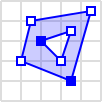
\includegraphics[width=0.2\textwidth]{figures/polygon_with_hole.png}}
        \hfill
\subfloat[Multipolygon]{\label{fig:a}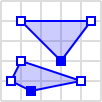
\includegraphics[width=0.2\textwidth]{figures/multipolygon.png}}
       \hfill
\subfloat[Multipolygon with hole]{\label{fig:a}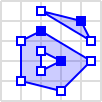
\includegraphics[width=0.2\textwidth]{figures/multipolygon_with_hole.png}}
    
    \caption{Three simple graphs}
    \label{fig:three graphs}
    
\end{figure}

\paragraph{Attributes}
Attributes are simply non-spatial data that's associated with the spatial data described above. An address, as mentioned above, is a great example of this: house numbers, streets, cities, states, and zip codes all associate an identifier with a point in space or other spatial concept~\cite{gentle_intro}.

\subsubsection{Raster}
Raster data is simply made up of grids of values. It's best to imagine a digital image: pixels arranged in a grid are each assigned red, green, and blue color values, and when they're appropriately combined and visualized, a continuous dataset is spread over a grid in two or three dimensions~\cite{gentle_intro}.

Images, in fact, are often raster data found in GISs, like satellite images. Atmospheric or ground sensors can also provide data sets that blanket an area~\cite{gentle_intro}.

Because raster data covers an area, programs and users need to account for the \textit{density} of data---that is, the size of each grid cell, which is referred to as the ``resolution.'' Resolution is either \textit{spatial} or \textit{spectral}:

\begin{description}
  \item[Spatial] Spatial resolution is how large a cell of the grid is and how it corresponds to a real geographic area. For example, a side of one cell could be four feet.
  \item[Spectral] Spectral resolution is the number of color ``bands'' in raster images. In an ordinary image, red, green, and blue are these three bands---the spectral resolution. In some cases, images may also capture infrared or ultraviolet light and store more data in other color bands.
\end{description}

\paragraph{Georeferencing}
Georeferencing makes raster data useful geographically: it associates the raster data with a location. For example, a GIS that displays a satellite image of California on top of an interactive state map can calculate where real geographic features are in the image~\cite{gentle_intro}.

As long as four pieces of information are known, a raster file can be properly georeferenced:

\begin{itemize}
  \item Coordinates of the file's top-left pixel
  \item Width of a pixel
  \item Height of a pixel
  \item Rotation of the grid
\end{itemize}

These four values will accurately positioned in a coordinate system~\cite{gentle_intro}.

\subsection{Abstract Specification}
OGC's Abstract Specification describes and standardizes the essential components of geospatial data, including the central information model and glossary for all OGC Standards~\cite{AbstractSpecFaq}.

Any sizable geospatial software system is naturally governed by certain geographic and geometric properties and functions; the Abstract Specification is the OGC's formalization of those concepts, all of which are encompassed in the data types and formats above and below~\cite{AbstractSpecFaq}.

\section{Data storage}
This section overviews several storage considerations for GIS data.

\subsection{Geospatial database management systems}
Because of the unique data considerations described earlier, databases that manage geospatial data need to pay special attention to the methods of doing so. Geospatial database management systems (GDBMSs) provide ways of storing and querying geospatial data. This includes syntax for adding vector and raster data types.

\paragraph{Example}
\label{background_wkt}
Inserting geometries (vector data) into a GDBMS can look like the following. We are using a SQL statement to add a point, linestring, polygon, and polygon with a hole to a PostGIS database (RAPID's underlying DBMS).

Note that space-separated numbers are a coordinate pair. The commas separate the points, creating an ordered series. This particular syntax is Well-Known Text (WKT), an OGC Standard for defining Abstract Specification geometries~\cite{ogc}. The five geometric data types correspond to the types described above in Section~\ref{sec:vector}.

\begin{Verbatim}[samepage=true,baselinestretch=1,numbers=left,xleftmargin=12mm]
CREATE TABLE geometries
 (name varchar, geom geometry);

INSERT INTO geometries VALUES
  (`Point',
   `POINT(0 0)'),
  (`Linestring',
   `LINESTRING(0 0, 1 1, 2 1, 2 2)'),
  (`Polygon',
   `POLYGON((0 0, 1 0, 1 1, 0 1, 0 0))'),
  (`PolygonWithHole',
   `POLYGON((0 0, 10 0, 10 10, 0 10, 0 0),
   (1 1, 1 2, 2 2, 2 1, 1 1))'),
  (`Collection',
   `GEOMETRYCOLLECTION(POINT(2 0),
   `POLYGON((0 0, 1 0, 1 1, 0 1, 0 0)))');

SELECT name, ST_AsText(geom)
FROM geometries;
\end{Verbatim}

These SQL statements demonstrate the creation of four geometries in a geospatial database: a single point, multiple connected strings, polygons with and without holes, and a generic collection of some of those same types.

\subsubsection{Querying}
An OGC Standard for querying geometries, Simple Feature Access (ISO 19125)~\cite{}, defines several required methods for comparing and relating them:

\begin{description}
  \item[Equals] Tests for equality of two geometries.
  \item[Intersects] Tests whether the interiors of geometries intersect.
  \item[Disjoint] The opposite of intersection.
  \item[Cross] Tests if the intersection of two geometries is in one dimension fewer than the source geometries.
  \item[Overlap] Determines if the intersection of two geometries is different from both the source geometries but of the same dimension.
  \item[Touch] Tests whether geometries have their boundaries touching (without intersected interiors).
  \item[Within and Contains] Test if a geometry is fully inside of another.
  \item[Distance] Calculates the shortest distance between two geometries.
  \item[DWithin] Tests whether objects are within a specified distance of each other.
\end{description}

It's easy to see where and why these come in handy. As a simple example, imagine that a mobile device stores its geographic location---a point---and is trying to determine the city it's currently in. If a GDBMS stores borders (polygons) for cities, a query can be performed that asks if the point is contained within cities' borders.

The queries below show some functions that are unique to geospatial data: the first selects the neighborhood(s) that the Broad Street subway station is located in, and the second selects points of interest within 1609 meters of any road.

\begin{Verbatim}[samepage=true,baselinestretch=1,numbers=left,xleftmargin=12mm]
SELECT nyc_subways.name, nyc_neighborhoods.name
FROM nyc_neighborhoods
JOIN nyc_subways
ON ST_Contains(nyc_neighborhoods.geom, nyc_subways.geom)
WHERE subways.name = 'Broad St';
\end{Verbatim}

\begin{Verbatim}[samepage=true,baselinestretch=1,numbers=left,xleftmargin=12mm]
SELECT roads.roadname, pois.poiname
FROM roads
JOIN pois 
ON ST_DWithin(roads.geom, pois.geom, 1609);
\end{Verbatim}

This type of analysis can be done application-side (as opposed to in the database) but GDBMS technologies have advanced enough that this type of data can be stored and queried very efficiently, with user-friendly queries that quickly and simply answer questions like the above one.

\subsection{Files}
\label{background_formats}
As can generally be the case with file formats and proprietary or fragmented software, geographic file formats are numerous and varied. Several formats come from cartographic- and surveillance-focused government agencies, like the United States Geological Survey and the National Geospatial-Intelligence Agency. Other particular GIS applications may have their own file considerations and requirements.

\subsubsection{Esri Shapefiles}
A go-to file format for vectors is Esri's shapefile, which includes the two vector features described above, attributes and point data.

Despite its singular name, a ``Shapefile'' is actually a set of several different file types:

\begin{description}
  \item[\tt{.shp}] These files contain the actual shape geometries.
  \item[\tt{.dbf}] These files store the non-spatial attributes that are associated with the geometries in the shapes file.
  \item[\tt{.shx}] These are index files that store metadata about entries' locations in a file and allow for seeking forward and backward between ordered ``features'' (shapes associated with their attributes).
\end{description}

Shapefiles are a mostly open and standard format managed and developed by Esri for use within the GIS space (and particularly their popular software, ArcGIS). Although this isn't an OGC Standard, it's become a ubiquitous vector format for GISs.

Interestingly, shapefiles have begun to show their age (they originated in the early 1990s), and there were calls for a more modern, robust shapefile format from the OGC, which resulted in GeoPackage, a modern vector format based on SQLite. Shapefile's ubiquity and history keeps it in widespread use, however ~\cite{slashgeo,GeoPackage}.

\subsubsection{GeoJSON}
GeoJSON is another common vector file format, although it's not standardized by OGC. It stores data in a nicely-readable format---a superset of JSON (JavaScript Object Notation). Take this example of a geospatial feature in GeoJSON:

\begin{Verbatim}[samepage=true,baselinestretch=1,numbers=left,xleftmargin=12mm]
{ "type": "Feature",
    "bbox": [-180.0, -90.0, 180.0, 90.0],
    "geometry": {
      "type": "Polygon",
      "coordinates": [[[-180.0, 10.0], [20.0, 90.0],
                       [180.0, -5.0], [-30.0, -90.0]]]
    }
}
\end{Verbatim}

It should be apparent that this syntax corresponds closely to the Abstract Specification we've been discussing, with standardized geometry types notated by series of points (latitudes and longitudes in this specific case).\footnote{This is the same OGC WKT format described in~\ref{background_wkt}.} Arbitrary, case-specific attributes can be appended in the same fashion as the key-value pairs above.

\paragraph{Bounding box}
The \textit{bbox} attribute is a \textit{bounding box}, which serves as an approximate area---bounding, rectangular dimensions---for a geospatial feature. Although actual feature coordinates may describe a more intricate border, a rougher bounding box is less complex and more efficient to compute spatial queries for. A bounding box may be a good-enough replacement for spatial queries that would normally be much slower. In some cases, it's reasonable to check spatial queries on bounding boxes and, if there's a match, then check the true geometry to confirm.\footnote{We discuss these tradeoffs in Section~\ref{validation_bbox}.}

A bounding box is not unique to GeoJSON and is commonly found in geospatial data specifications and APIs.

\subsubsection{Related formats}
There are dozens of other geospatial file formats with certain specializations, degrees of standardization, and application-specific features, but Shapefiles and GeoJSON are nicely representative of their general capabilities and stylistic differences.